\documentclass{beamer}
\usetheme{Copenhagen}
\usecolortheme{seahorse}
\usefonttheme[onlymath]{serif}

\usepackage{setspace}
\usepackage{xcolor}
\usepackage{graphicx}
\usepackage{multimedia}
\usepackage{fontawesome5}
\usepackage[most]{tcolorbox}
\usepackage{empheq}
\usepackage{fancybox}
\usepackage{annotate-equations}
\usepackage{tikz}
\usetikzlibrary{positioning, calc, shapes.geometric, shapes.multipart, 
	shapes, arrows.meta, arrows, 
	decorations.markings, external, trees}
\tikzstyle{Arrow} = [
thick, 
decoration={
	markings,
	mark=at position 1 with {
		\arrow[thick]{latex}
	}
}, 
shorten >= 3pt, preaction = {decorate}
]

\definecolor{teel}{HTML}{00AEB3}
\definecolor{redorange}{HTML}{F26035}
\definecolor{ForestGreen}{RGB}{34,139,34}
\definecolor{darkgreen}{HTML}{06402B}
\definecolor{CarolinaBlue}{HTML}{4B9CD3}
\usecolortheme[named=CarolinaBlue]{structure}


\title[Random Seeds]{Stabilizing Causal Estimates: Tackling Random Seed Dependence in Machine Learning}
\author[Paul Zivich]{Paul Zivich \\~\\ Assistant Professor \\ Department of Epidemiology \\ Gillings School of Global Public Health \\ University of North Carolina at Chapel Hill}

\setbeamercovered{transparent}
\setbeamertemplate{navigation symbols}{}  % gets rid of the dumb navigation symbols
\setbeamertemplate{page number in head/foot}{\insertframenumber}  % adds slide #
\setbeamertemplate{headline}{}

\AtBeginSection[]{
	\begin{frame}
		\vfill
		\centering
		\begin{beamercolorbox}[sep=8pt,center,shadow=true,rounded=true]{title}
			\usebeamerfont{title}\insertsectionhead\par%
		\end{beamercolorbox}
		\vfill
	\end{frame}
}

\begin{document}
	
\begin{frame}[plain]
	\maketitle
\end{frame}

\begin{frame}{Acknowledgements\footnote[frame]{Footnotes are for asides or references, but fair game for questions}}
	\textbf{Funding}: K01AI177102 \\~\\
	\textbf{Disclaimer}: views are mine and not those of NIH, US gov \\~\\
	\textbf{Publication}: Zivich \textit{Epidemiology} 2024; 35(6):787-790. \\~\\
	\begin{center}
		\small
		\faEnvelope \quad pzivich@unc.edu \qquad \quad 
		\faGithub \quad pzivich \qquad \quad
		\faHashtag \quad pausalz@bsky.social
	\end{center}
\end{frame}

\begin{frame}{Steps for Causal Inference}
	Identification
	\begin{itemize}
		\item Translate parameter into observed data
		\item Machine learning unlikely to be helpful here
	\end{itemize}
	~\\~\\
	Estimation
	\begin{itemize}
		\item Use observed data expression to estimate the parameter
		\item Machine learning may be useful\footnote[frame]{Machine learning is not magic. Even data-adaptive algorithms can need variable pre-processing or transformations for validity. See Naimi, Mishler, \& Kennedy \textit{American Journal of Epidemiology} 2023}
	\end{itemize}
\end{frame}

\begin{frame}{Notation}
	$Y^a$: potential outcome under action $a$ \\~\\
	$Z = (W,A,Y)$ \\
	$Y$: outcome of interest \\
	$A$: action of interest \\
	$W$: covariate vector 
	\begin{itemize}
		\item $\mathcal{W}$ denotes the support
	\end{itemize}
	~\\
	\textbf{Parameter}: average causal effect
	$$ \psi = E[Y^1 - Y^0] $$	
\end{frame}

\begin{frame}{Identification}
	Express parameter of interest as a function of the observed data
	~\\~\\~\\
	Given causal consistency, exchangeability by $W$ with positivity
	\[ \psi = E\left[ E(Y \mid A=1, W) \right] - E\left[ E(Y \mid A=0, W) \right] \]
\end{frame}

\begin{frame}{Estimation\footnote[frame]{Not all identified parameters are estimable, see Maclaren \& Nicholson 2021 or Aronow et al. 2025 \textit{Observational Studies}}}
	AIPW estimator
	\begin{equation*}
		\hat{E}[Y^a] = \frac{1}{n} \sum_{i=1}^{n} \left\{ \mu(a, W_i) + \frac{I(A_i = a) \left[ Y_i - \mu(a, W_i)\right]}{\pi(W_i)} \right\}
	\end{equation*}
	where
	\[\pi(W) = \Pr(A=a \mid W)\]
	\[\mu(A, W) = E(Y \mid A, W)\]
	as $\pi$ and $\mu$ are unknown in observational research, need to be estimated instead
\end{frame}

%\begin{frame}{Low Dimensional $\mathcal{W}$}
%	Let $p$ denote the size of $\mathcal{W}$
%	~\\~\\
%	When $n > p$ can fit a saturated model for $\pi$ or $\mu$.\footnote[frame]{IPW, g-computation, AIPW are exactly equal with saturated models}
%	\begin{itemize}
%		\item No modeling constraints imposed
%		\item Estimation requires no additional assumptions
%	\end{itemize}
%\end{frame}
%
%\begin{frame}{High Dimensional $\mathcal{W}$}
%	Often that $n << p$ in practice
%	\begin{itemize}
%		\item Saturated models no longer possible
%	\end{itemize}
%	~\\
%	Model to borrow information from `nearby' observations
%	\begin{itemize}
%		\item Borrowing does not come free
%		\item Validity relies on specification of model enabling borrowing
%	\end{itemize}
%	~\\
%	\begin{block}{Correct Model Specification}
%		\begin{equation*}
%			\Pr(A=a \mid W) \in \mathcal{M}_{\alpha} = \{\pi(W; \alpha) : \alpha \in A \} 
%		\end{equation*}
%		\begin{equation*}
%			E[Y \mid A,W] \in \mathcal{M}_{\beta} = \{\mu(A,W; \beta) : \beta \in B \} 
%		\end{equation*}
%	\end{block}
%\end{frame}

\begin{frame}{Dimension of $\mathcal{W}$}
	Let $p$ denote the size of $\mathcal{W}$
	~\\~\\
	When $n > p$ can fit a saturated model for $\pi$ or $\mu$.\footnote[frame]{IPW, g-computation, AIPW are exactly equal with saturated models}
	\begin{itemize}
		\item No modeling constraints imposed
	\end{itemize}
	~\\
	Often that $n << p$ in practice
	\begin{itemize}
		\item Model to borrow information from `nearby' observations
	\end{itemize}
	~\\
	\begin{block}{Correct Model Specification}
		\begin{equation*}
			\Pr(A=a \mid W) \in \mathcal{M}_{\alpha} = \{\pi(W; \alpha) : \alpha \in A \} 
		\end{equation*}
		\begin{equation*}
			E[Y \mid A,W] \in \mathcal{M}_{\beta} = \{\mu(A,W; \beta) : \beta \in B \} 
		\end{equation*}
	\end{block}
\end{frame}

\begin{frame}{Parametric Models}
	\begin{center}
		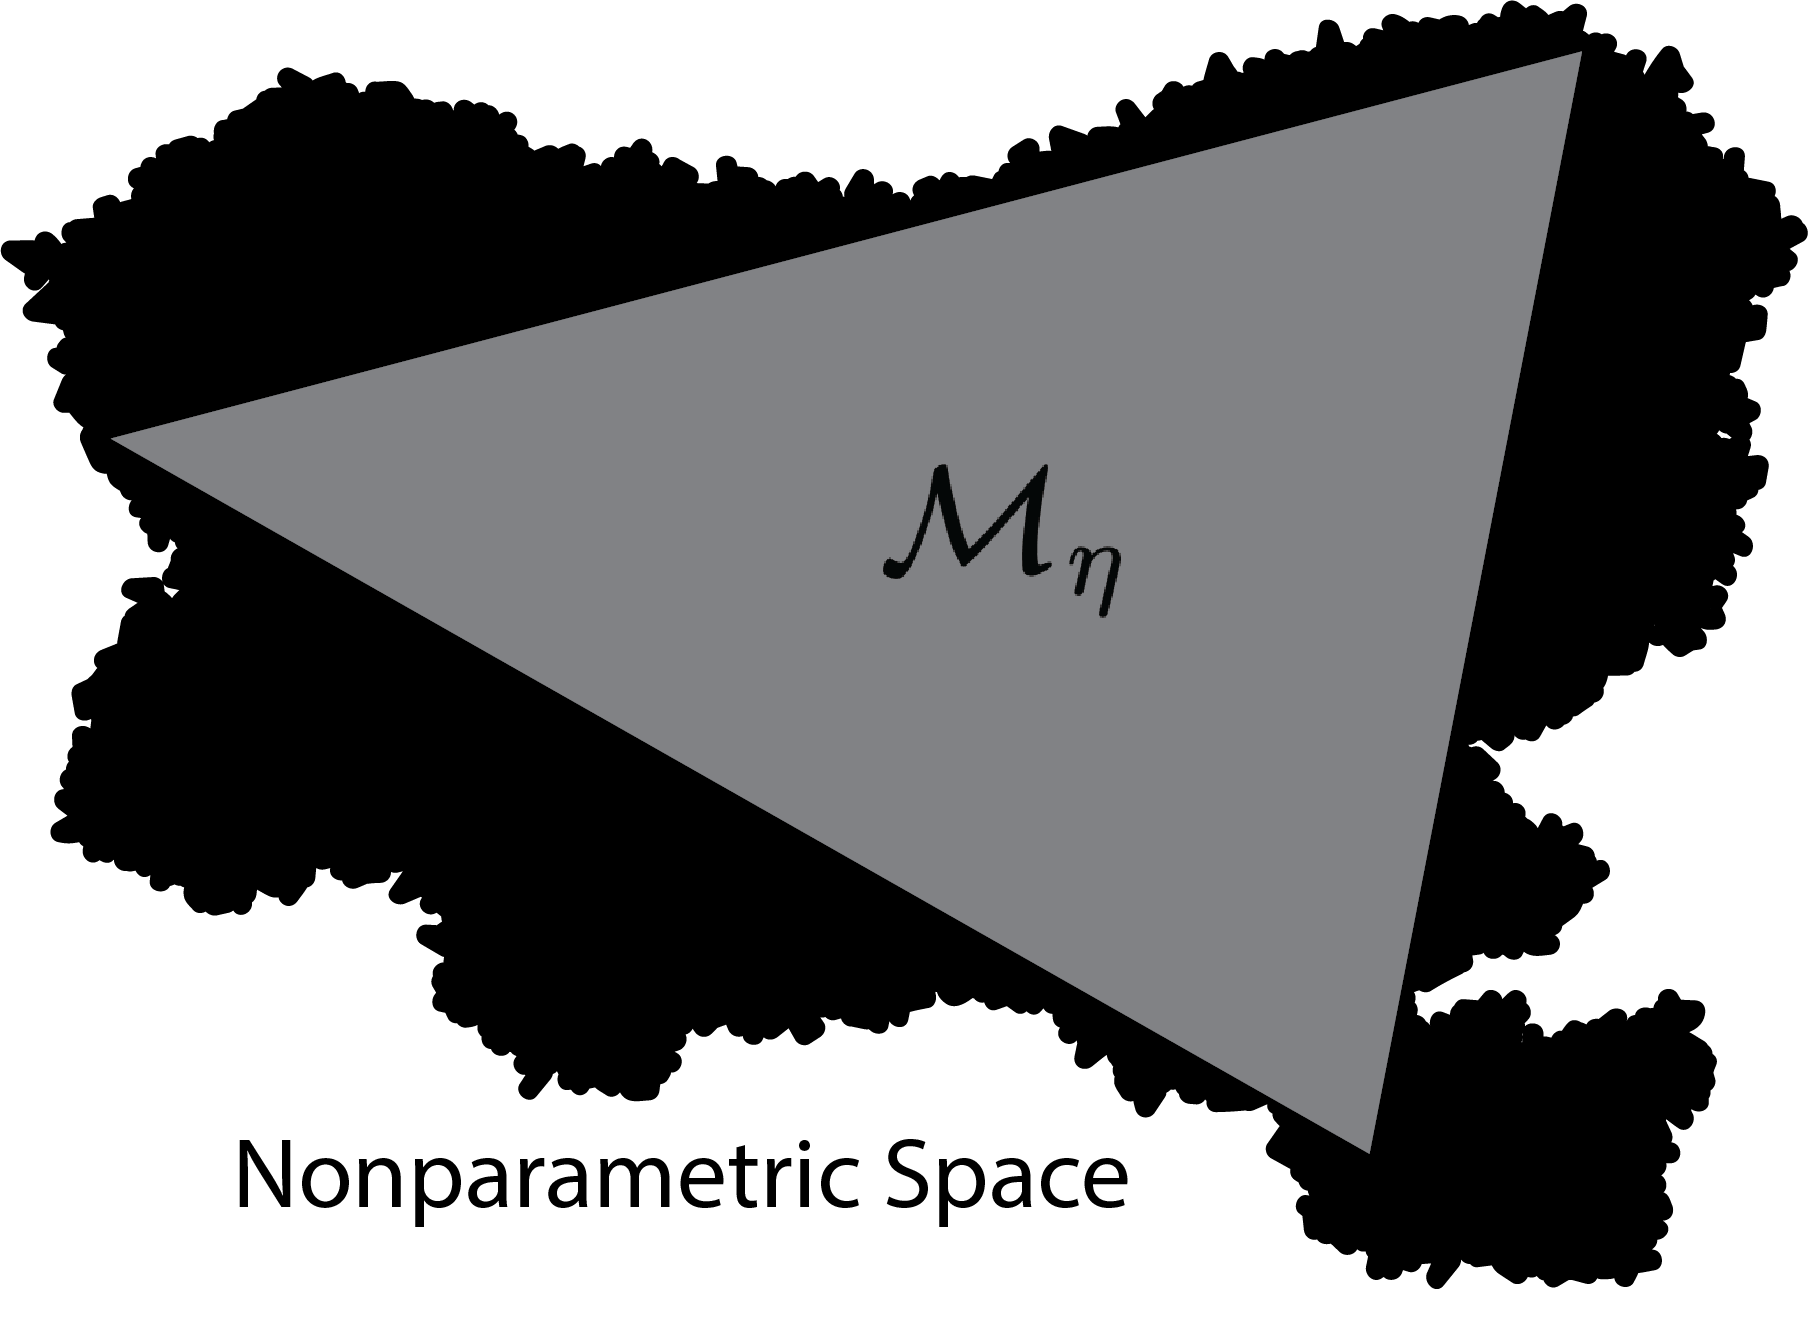
\includegraphics[width=0.95\linewidth]{images/model_parametric.png}
	\end{center}
\end{frame}

\begin{frame}{Data-Adaptive Models} 
	\begin{center}
		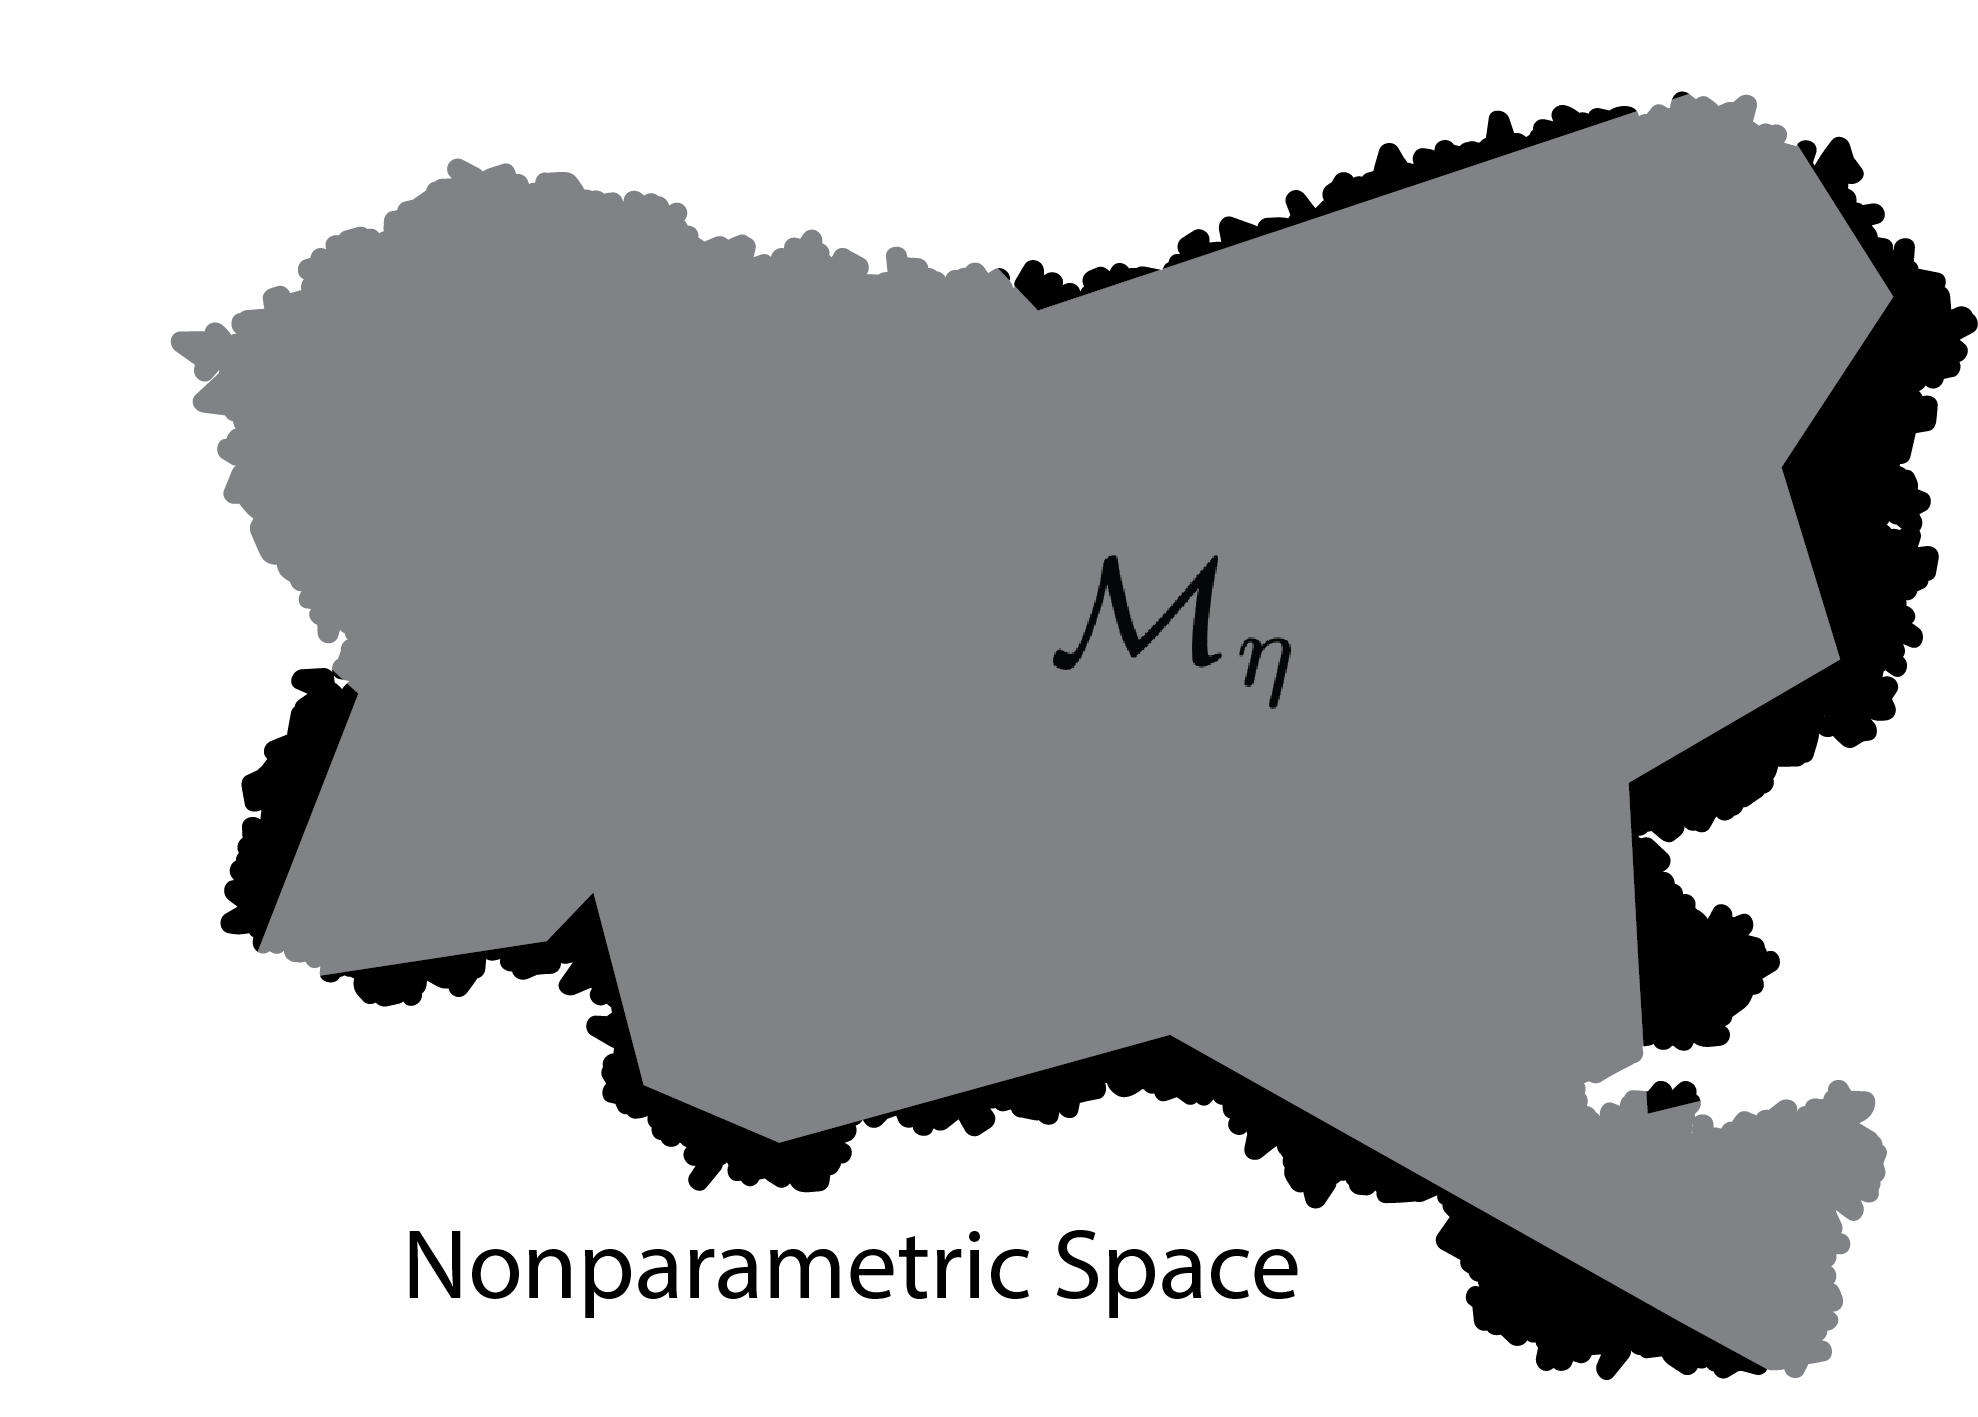
\includegraphics[width=0.95\linewidth]{images/model_nonparametric.png}
	\end{center}
\end{frame}

\begin{frame}{Challenges for Theory}
	Wider class does not come freely\footnote[frame]{Zivich et al. 2022 \textit{Wiley StatsRef}}
	\begin{itemize}
		\item[1.] Convergence rates\footnote[frame]{Daniel 2018 \textit{Wiley StatsRef}}
		\begin{itemize}
			\item \textbf{Solution}: rate-robust estimators (AIPW, TMLE)\footnote[frame]{Cost of rate-robustness is double-susceptibility to model misspecification}
		\end{itemize}
		\begin{equation*}
			\left[ \frac{1}{\hat{\pi}(W)} - \frac{1}{\pi(W)} \right] \times \left[ \hat{\mu}(A,W) - \mu(A,W) \right]
		\end{equation*}
		~\\
		\item[2.] Donsker class restriction\footnote[frame]{Chernozhukov et al. 2018 \textit{The Econometrics Journal}}
		\begin{itemize}
			\item \textbf{Solution}: cross-fitting
			\item Split into train-test set, fit nuisance models in train set and estimate effect in test set (then swap roles)
		\end{itemize}
	\end{itemize}
\end{frame}

\begin{frame}{Challenges for Practice}
	\begin{itemize}
		\item[1.] Computational complexity
		\item[2.] Algorithm selection
		\item[3.] Dependence on Random Number Generators (RNGs)
	\end{itemize}
\end{frame}

\section{(Pseudo) Random Number Generators}

\begin{frame}{(Pseudo) Random Number Generators}
	RNGs are deterministic functions that take a starting state
	\begin{itemize}
		\item Seed determines sequence of all generated numbers
		\item Changing the seed changes the sequence
	\end{itemize}
	~\\
	Role of RNGs in causal effect estimation with machine learning
	\begin{itemize}
		\item[1.] Machine learning algorithms
		\item[2.] Cross-validated stacking algorithms (e.g., super learner)
		\item[3.] Data splitting within cross-fitting
	\end{itemize}
\end{frame}

\begin{frame}{Illustration of Seed Dependence}
	\begin{center}
		same data set, same estimator, different seeds
		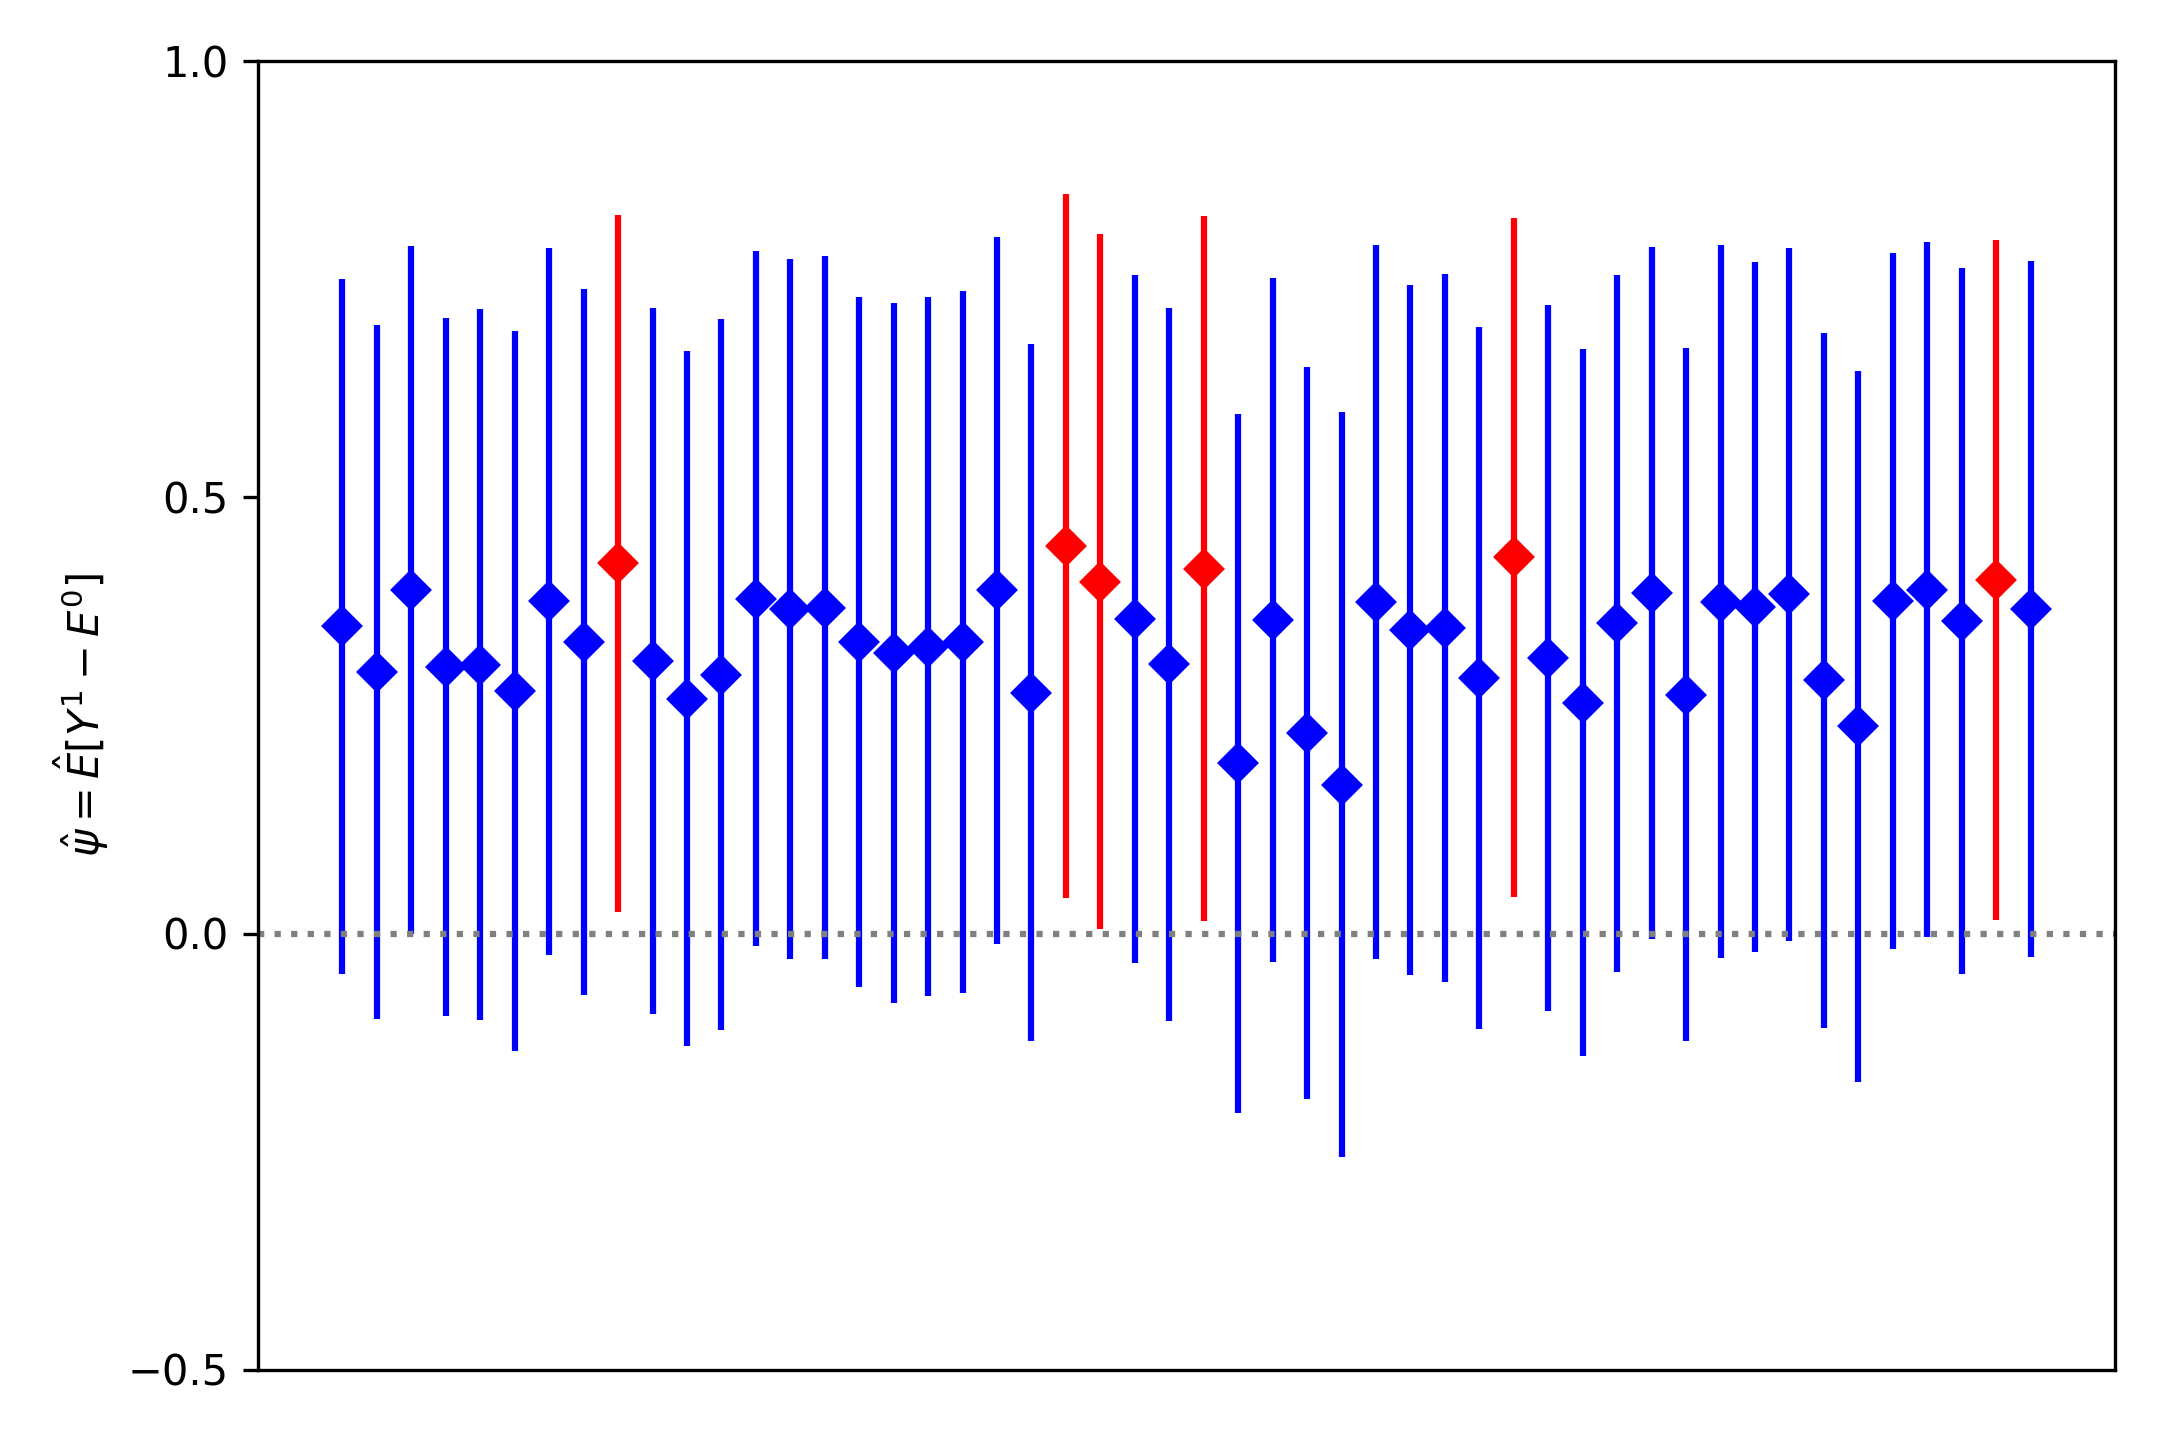
\includegraphics[width=0.95\linewidth]{images/data_example.png}
	\end{center}
\end{frame}

\begin{frame}{Seed Dependence is Unacceptable}
	Replicability
	\begin{itemize}
		\item Results not reproducible unless seed is known
	\end{itemize}
	~\\
	Offers a new version of p-hacking\footnote[frame]{Some have argued that seeds should be thought of as a hyperparameter that we should tune over (Bethard \textit{arXiv:2210.13393}). I strongly disagree as it is unclear what we are tuning over and this seems ripe for abuse, at least within a publish-or-perish system}
	\begin{itemize}
		\item Difficult to uncover
	\end{itemize}
	~\\
	Decision making should not depend on something arbitrary as a choice of seed for a RNG
\end{frame}

\begin{frame}{Solutions to Seed Dependence\footnote[frame]{Detailed in Schader et al. \textit{Epidemiology} 2024; Zivich \textit{Epidemiology} 2024}}
	Average $\pi$ and $\mu$ predictions under different seeds
	\begin{itemize}
		\item Hard to implement with cross-fitting
	\end{itemize}
	~\\
	Average $\hat{\psi}$ under different seeds
	\begin{itemize}
		\item Easy to implement
		\item Rubin's Rule for variance
	\end{itemize}
	~\\
	Increase number of folds within cross-fitting
	\begin{itemize}
		\item Applies to cross-fitting or cross-validation
	\end{itemize}
\end{frame}

\section{Simulations}

\begin{frame}{Data Generating Mechanism\footnote[frame]{Inspired by Weierstrass's continuous but non-differentiable functions}}
	Propensity score
	\begin{equation*}
		A \sim \text{Bernoulli} \left[ 0.75 - 1.2\left(\sum_{j=1}^{100} \frac{\sin(W_i \pi j^3)}{\pi j^3}\right)  \right]
	\end{equation*}
	Outcome model
	% (a**i) * np.cos(b**i * np.pi * x)
	\begin{equation*}
		Y^1_i \sim \text{Normal}\left[ 5 \times \left(\sum_{j=1}^{100} 0.5^j \cos(2 W_i 5^j \pi )\right), \sigma \right]
	\end{equation*}
	\begin{equation*}
		Y^0_i \sim \text{Normal}\left[ 5 \times \left(\sum_{j=1}^{100} 0.5^j \cos(W_i 5^j \pi )\right), \sigma \right]
	\end{equation*}
	where $\sigma = 1$
\end{frame}

\begin{frame}{Data Generating Mechanism}
	\begin{center}
		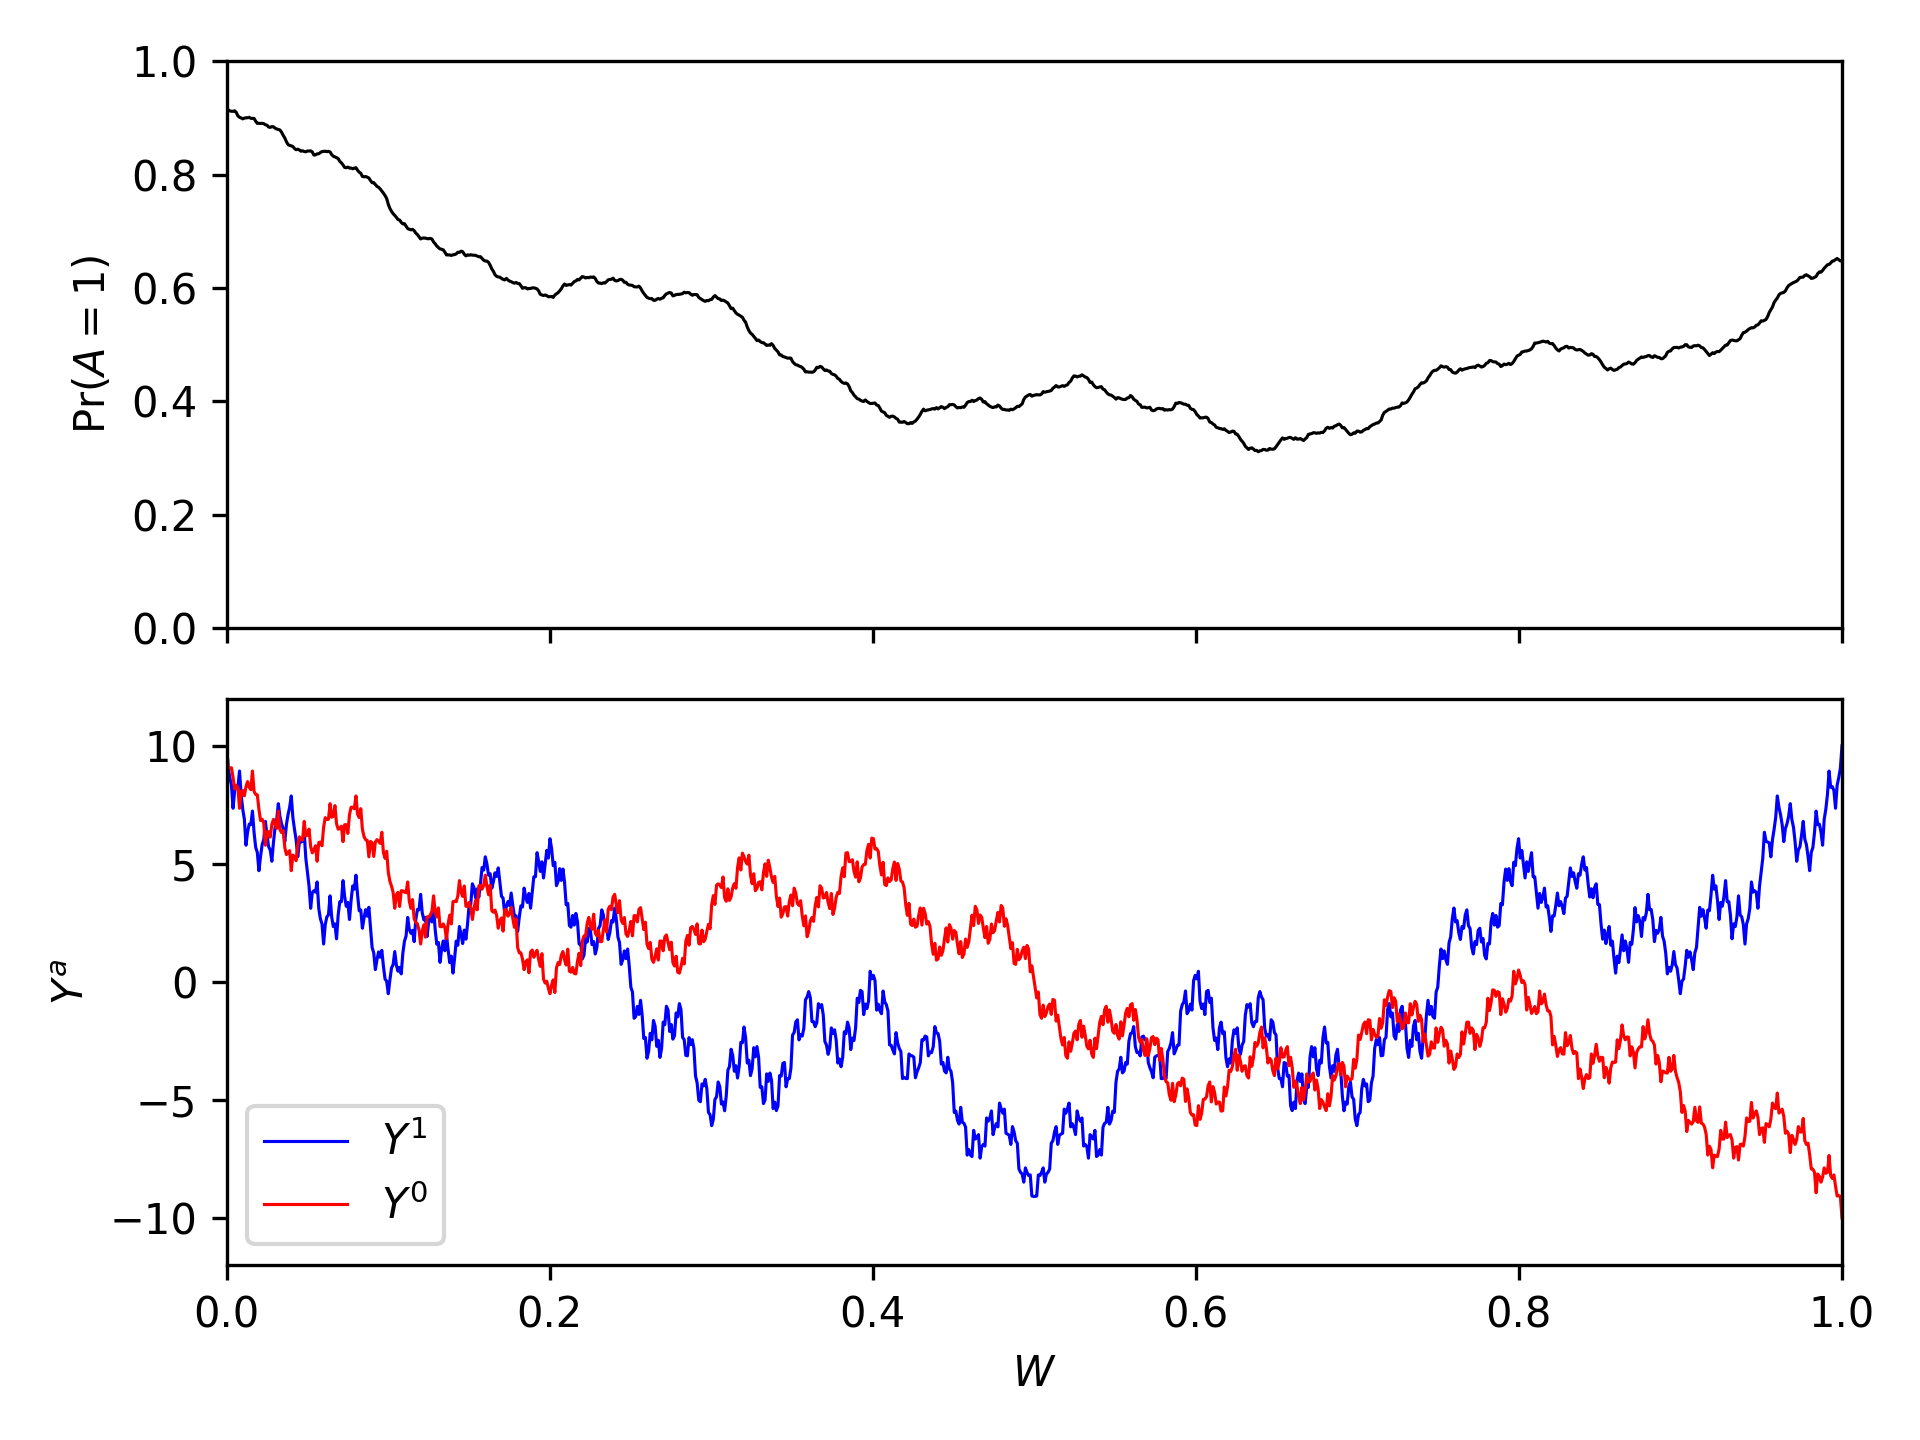
\includegraphics[width=0.95\linewidth]{images/dgm.png}
	\end{center}
\end{frame}

\begin{frame}{Single Cross-Fit Targeted Maximum Likelihood Estimator}
	\begin{center}
		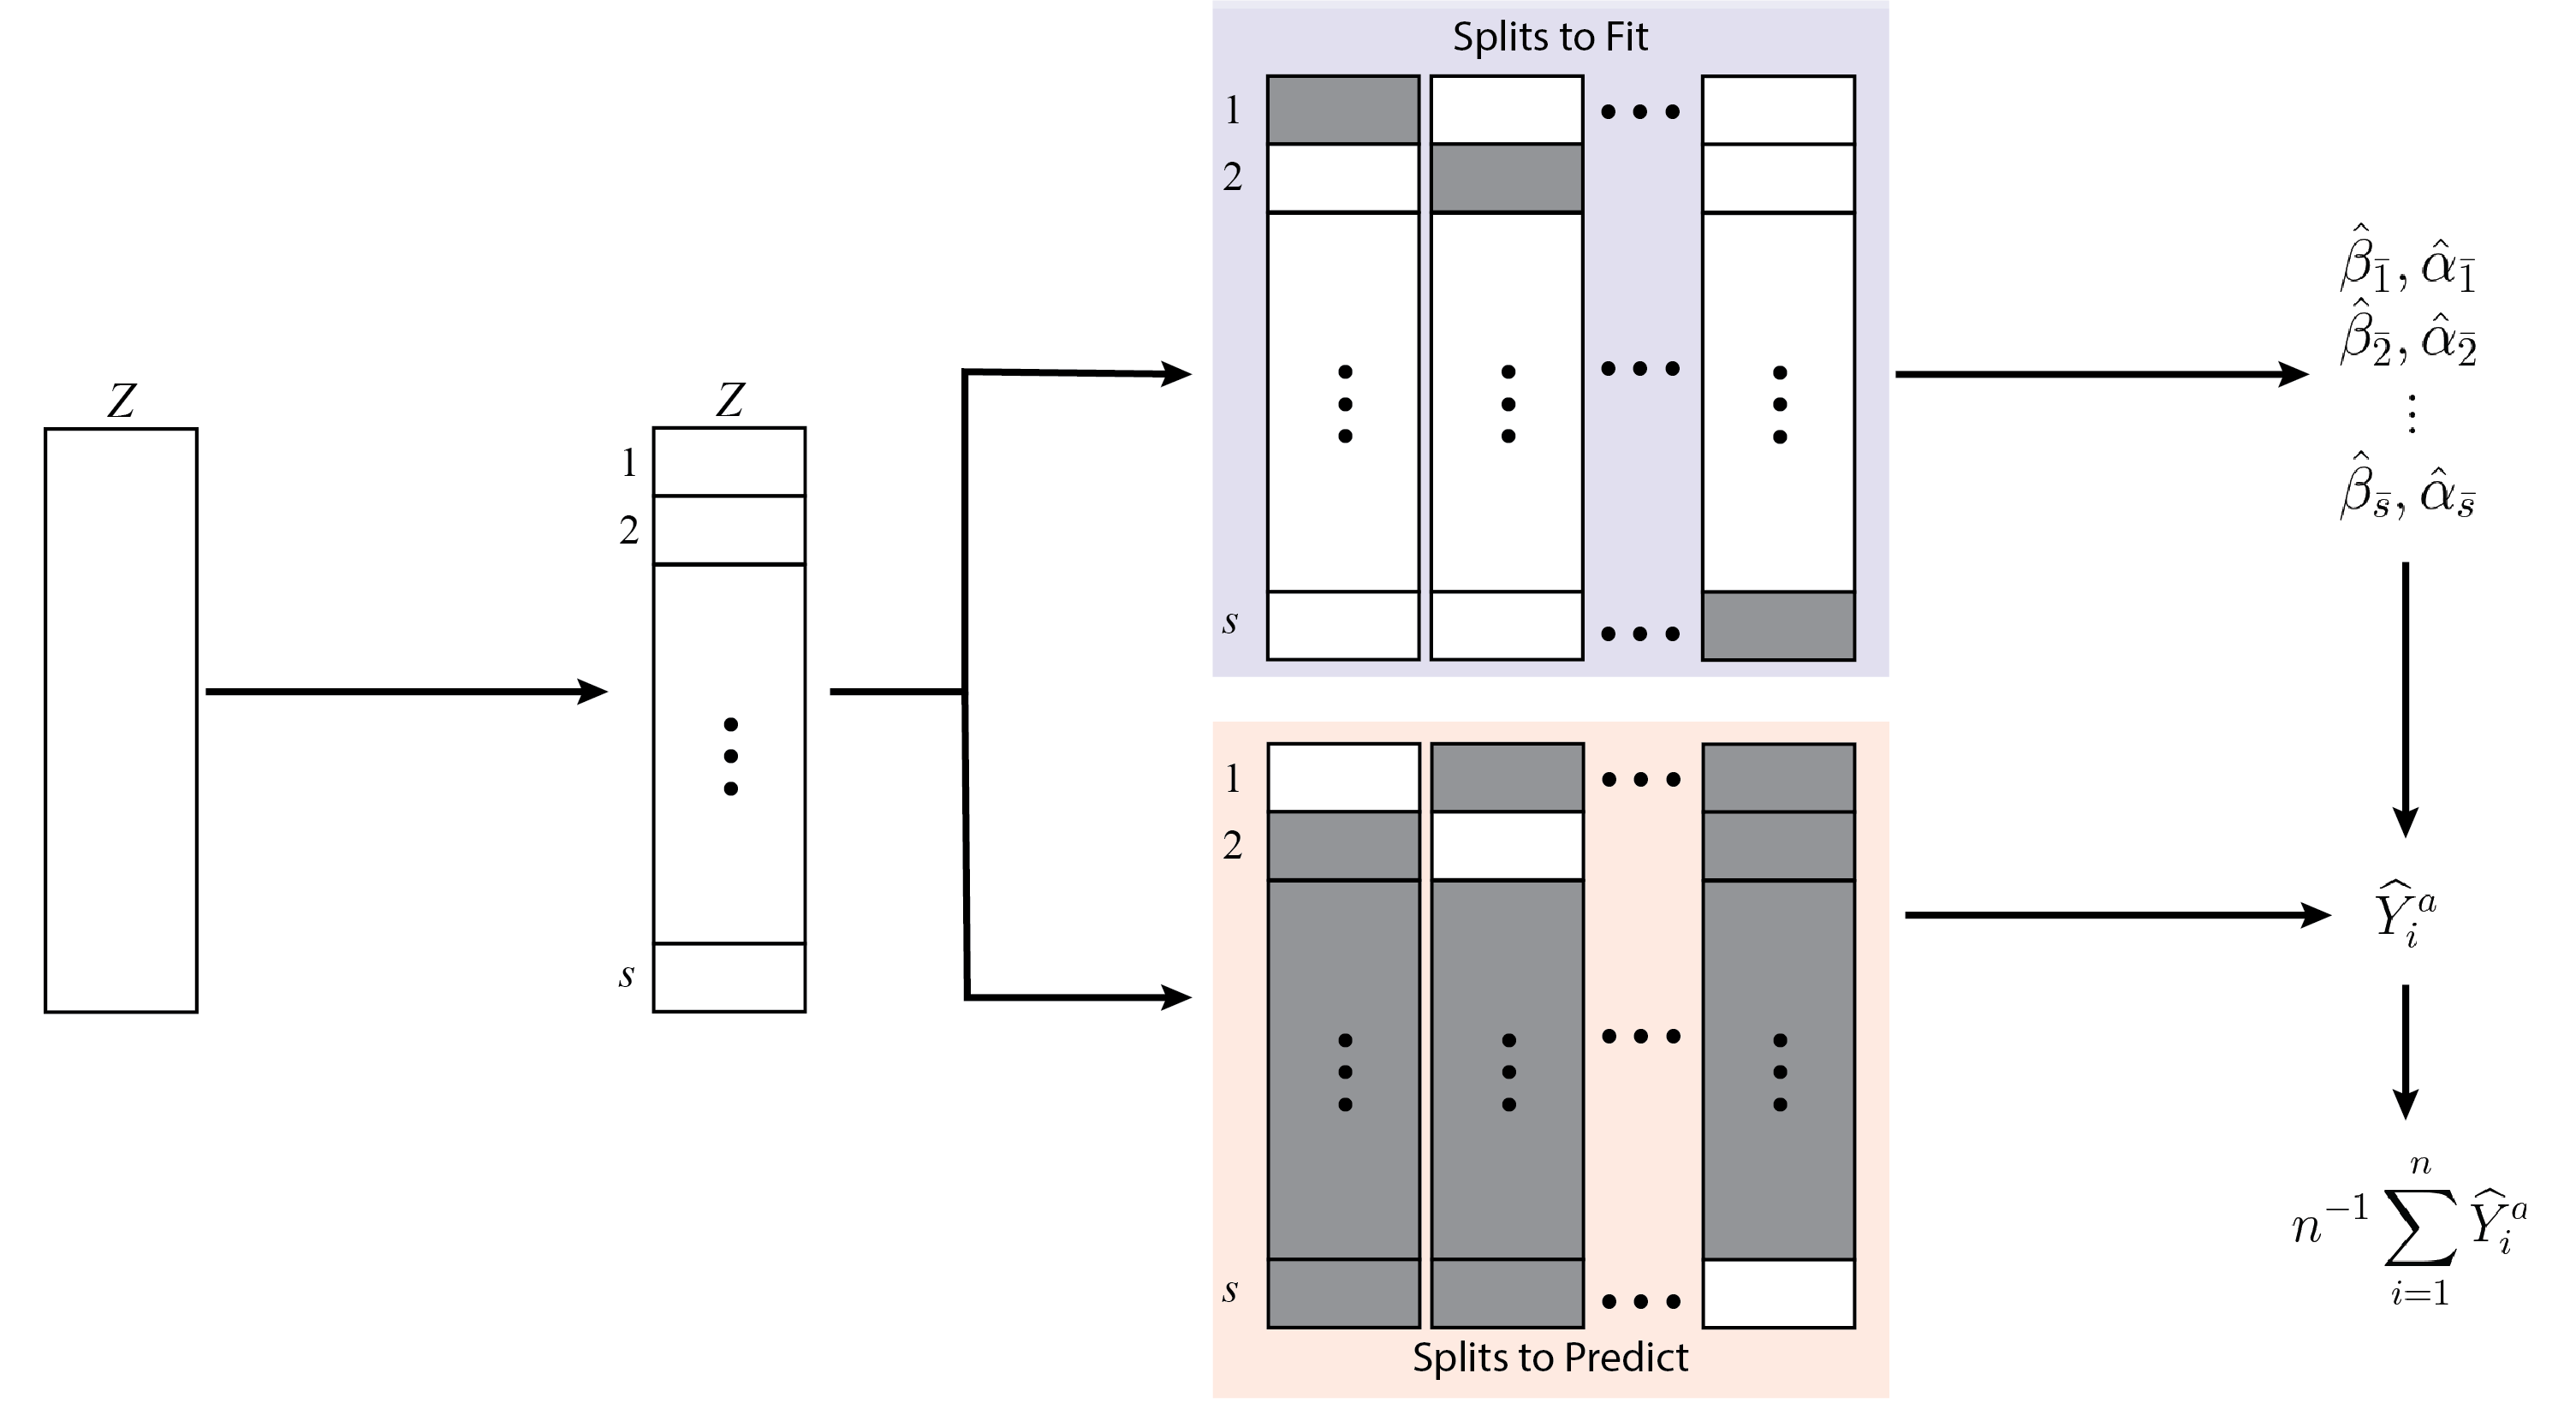
\includegraphics[width=0.8\linewidth]{images/cross-fitting.png}
	\end{center}
	Super learner\footnote[frame]{Neural network was favored for $\pi$. Decision tree was favored for $\mu$}
	\begin{itemize}
		\item Generalized linear model, cross-validated LASSO, decision tree, 4-layer neural network
	\end{itemize}
\end{frame}

\begin{frame}{Process}
	\begin{itemize}
		\item Generate $n=1000$ observations
		\item Apply SCFTMLE under 50 different randomly chosen seeds
		\item Compute standard deviation (SD) of point and standard error estimates\footnote[frame]{Exactly zero for parametric estimators}
		\item Repeat 200 different data sets
	\end{itemize}
	~\\
	Metrics
	\begin{itemize}
		\item Mean of SD of point and standard error estimates
	\end{itemize}
\end{frame}

\begin{frame}{Variations in SCFTMLE}
	\begin{center}
		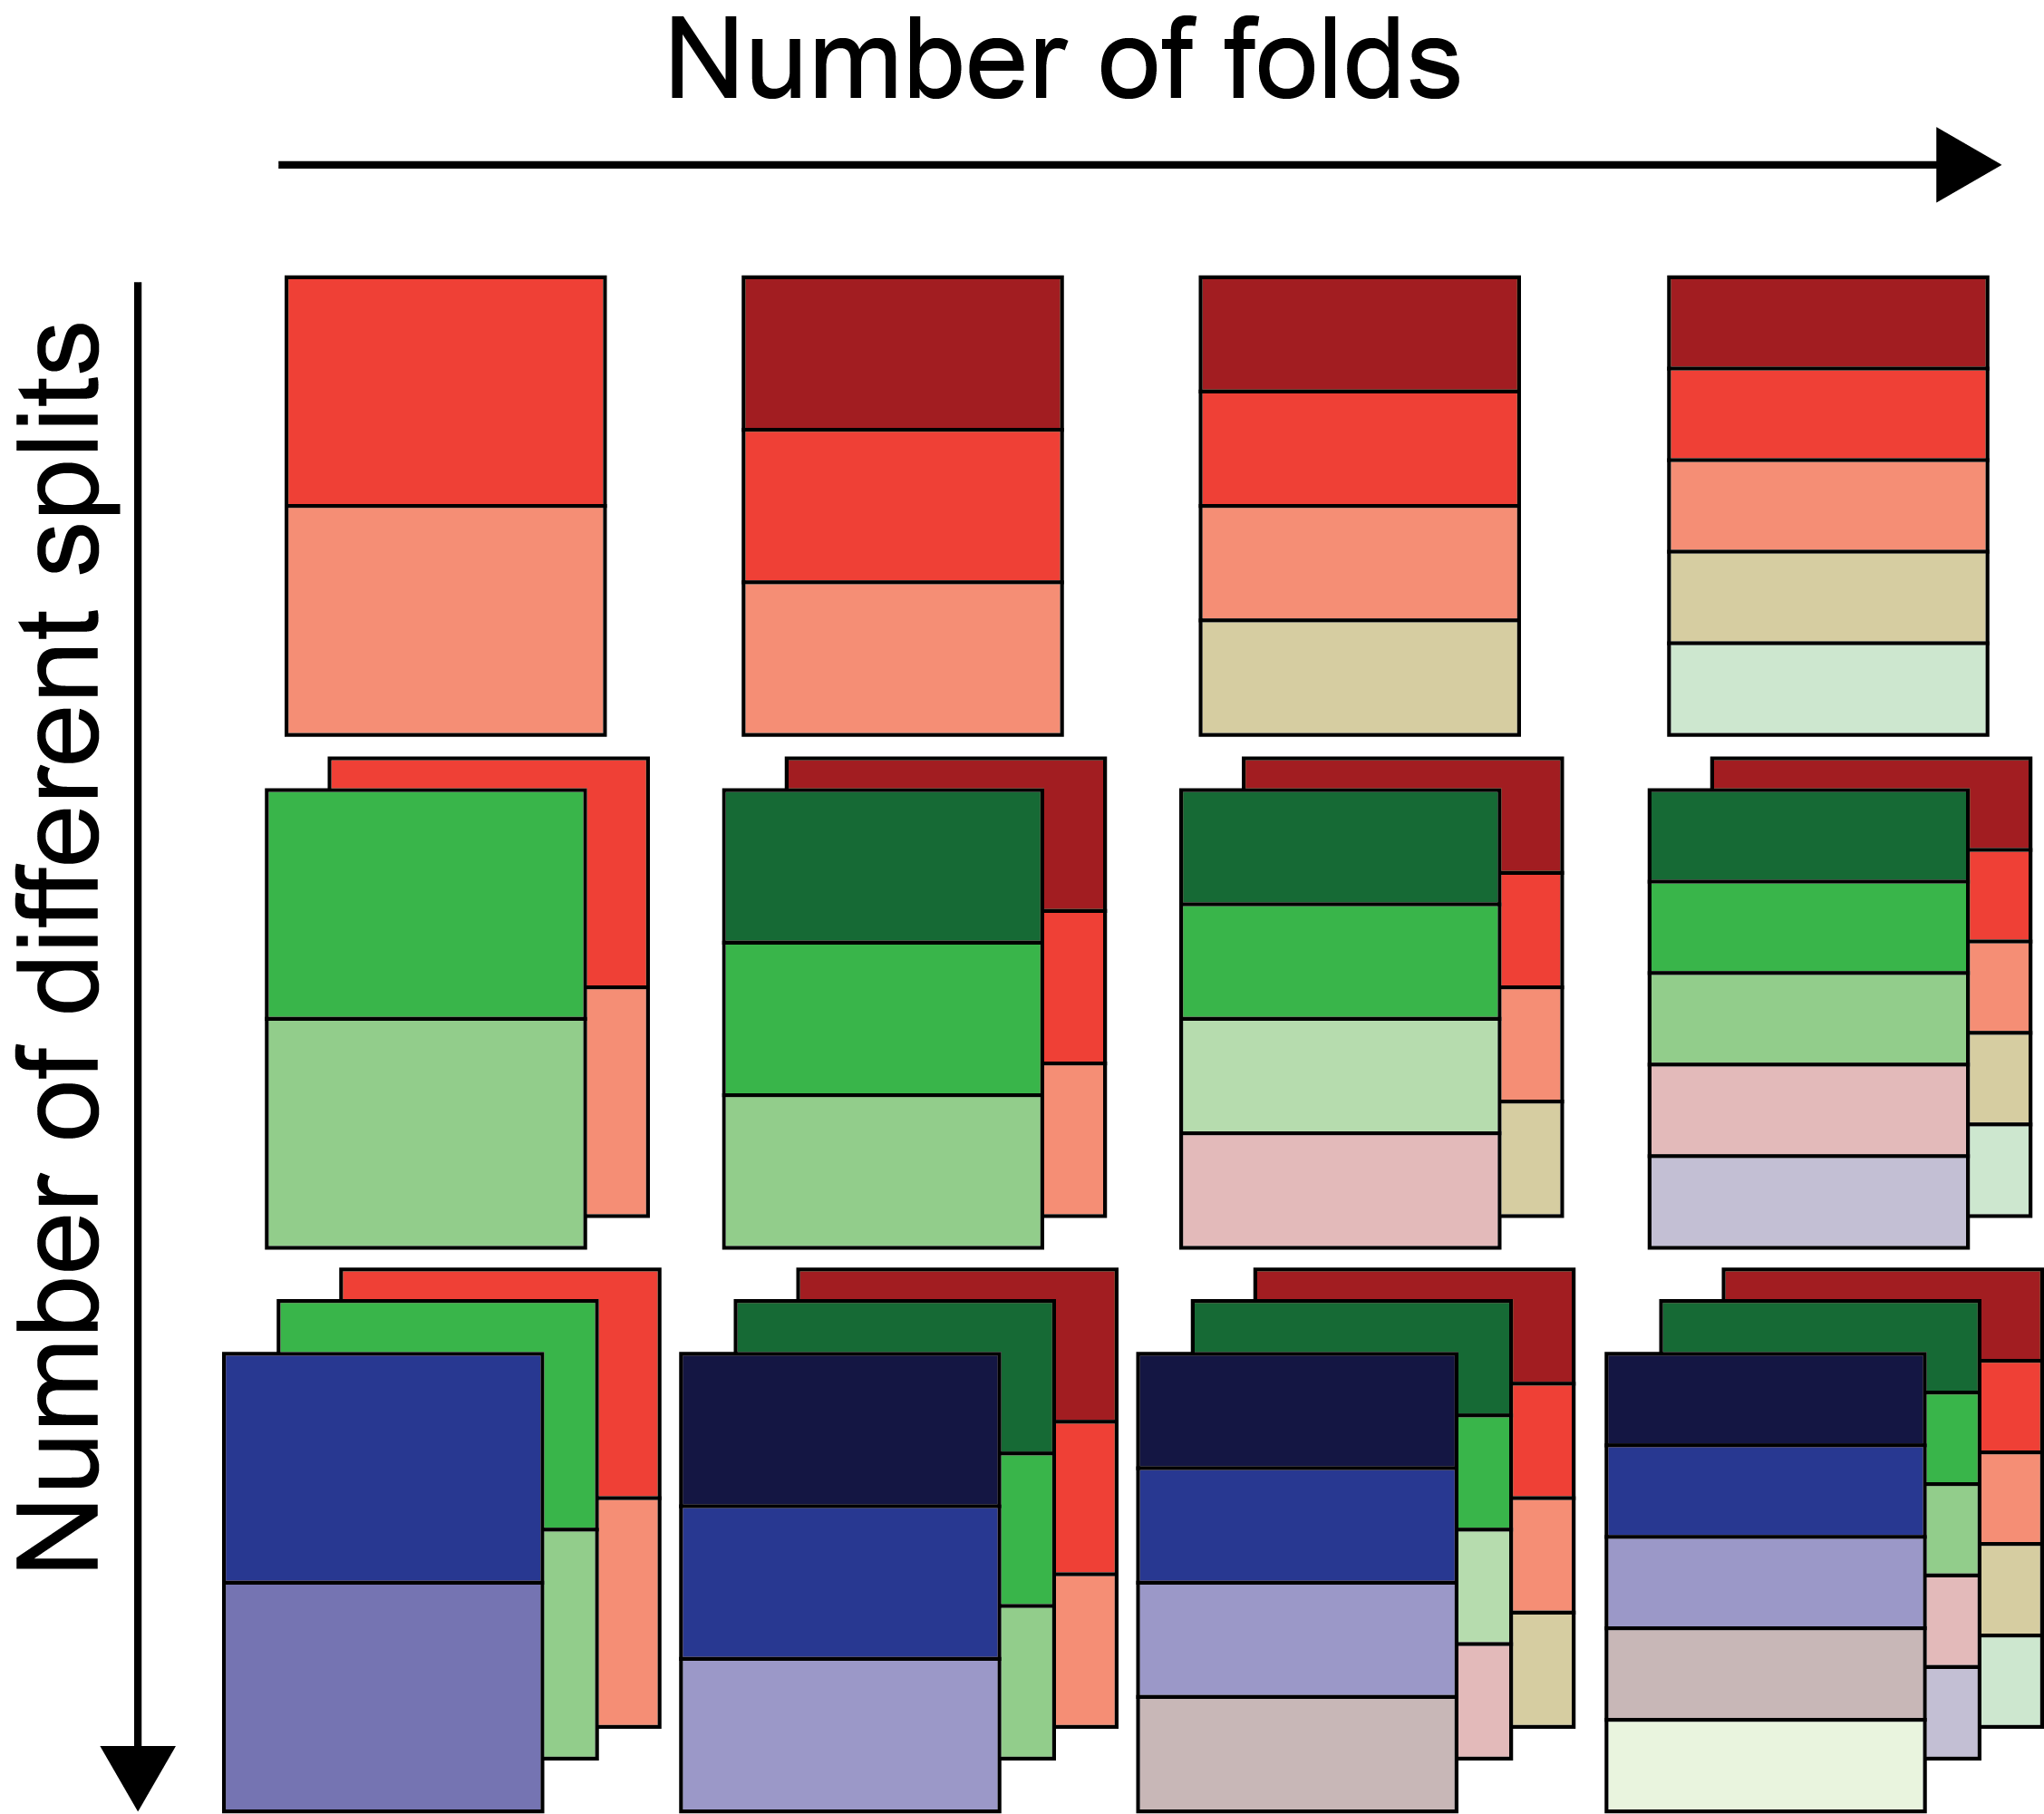
\includegraphics[width=0.72\linewidth]{images/variations.png}
	\end{center}
\end{frame}

\begin{frame}{Results -- Illustration for Single Data Set}
	\begin{center}
		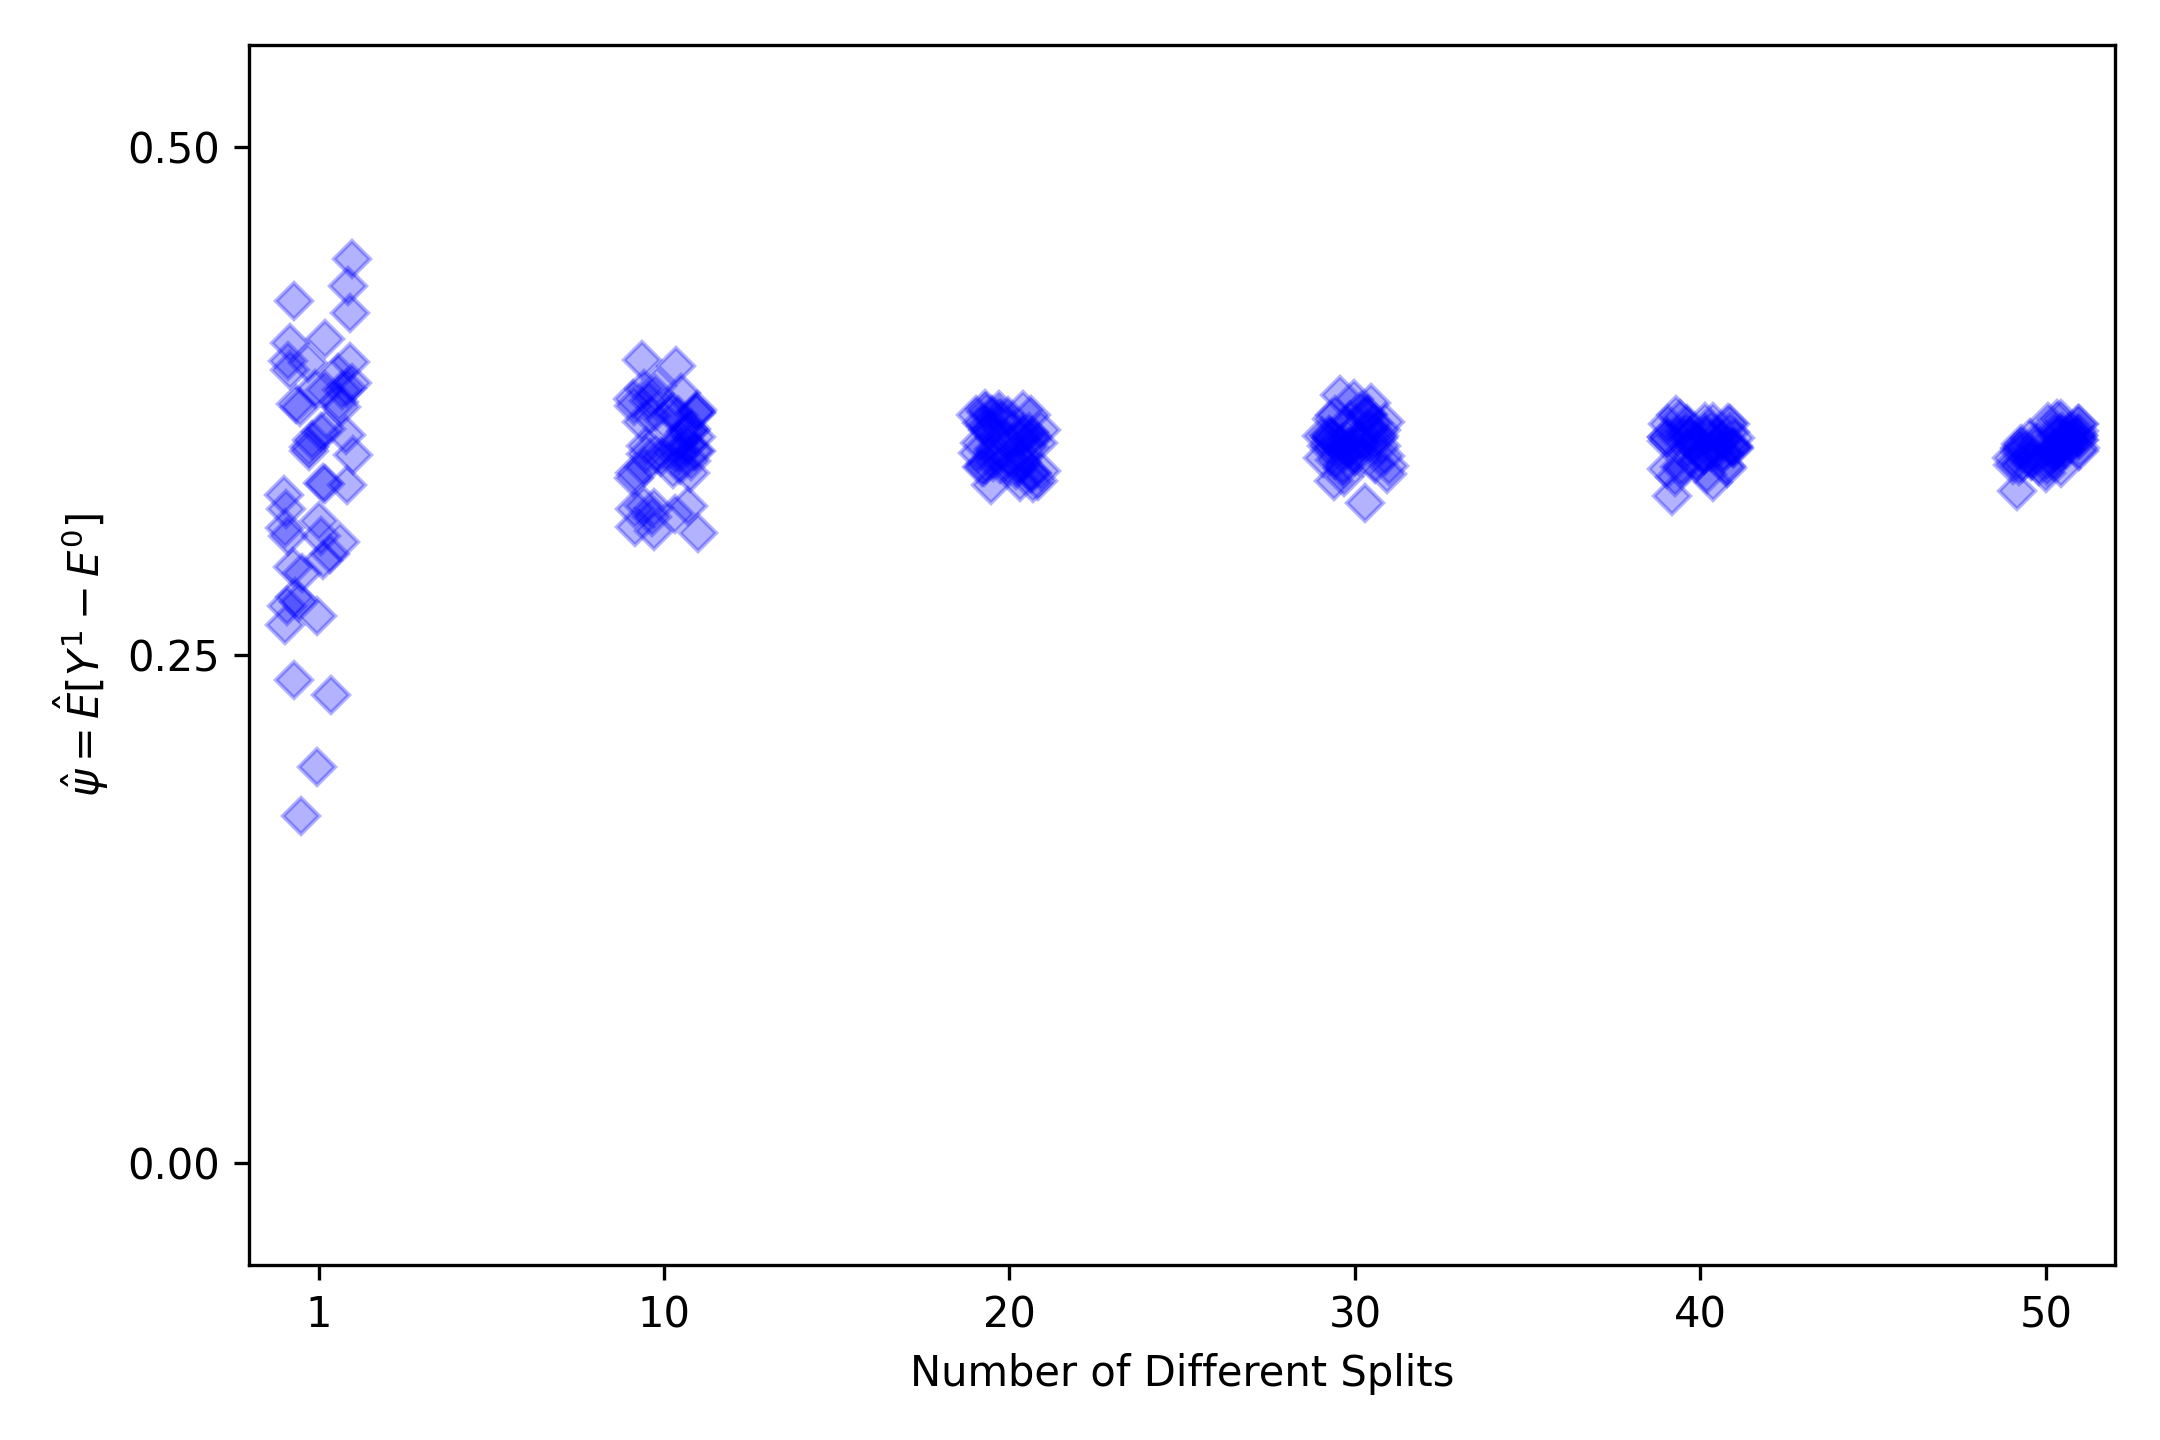
\includegraphics[width=0.99\linewidth]{images/data_example_splits.png}
	\end{center}
\end{frame}

\begin{frame}{Results -- Point Estimate}
	\begin{center}
		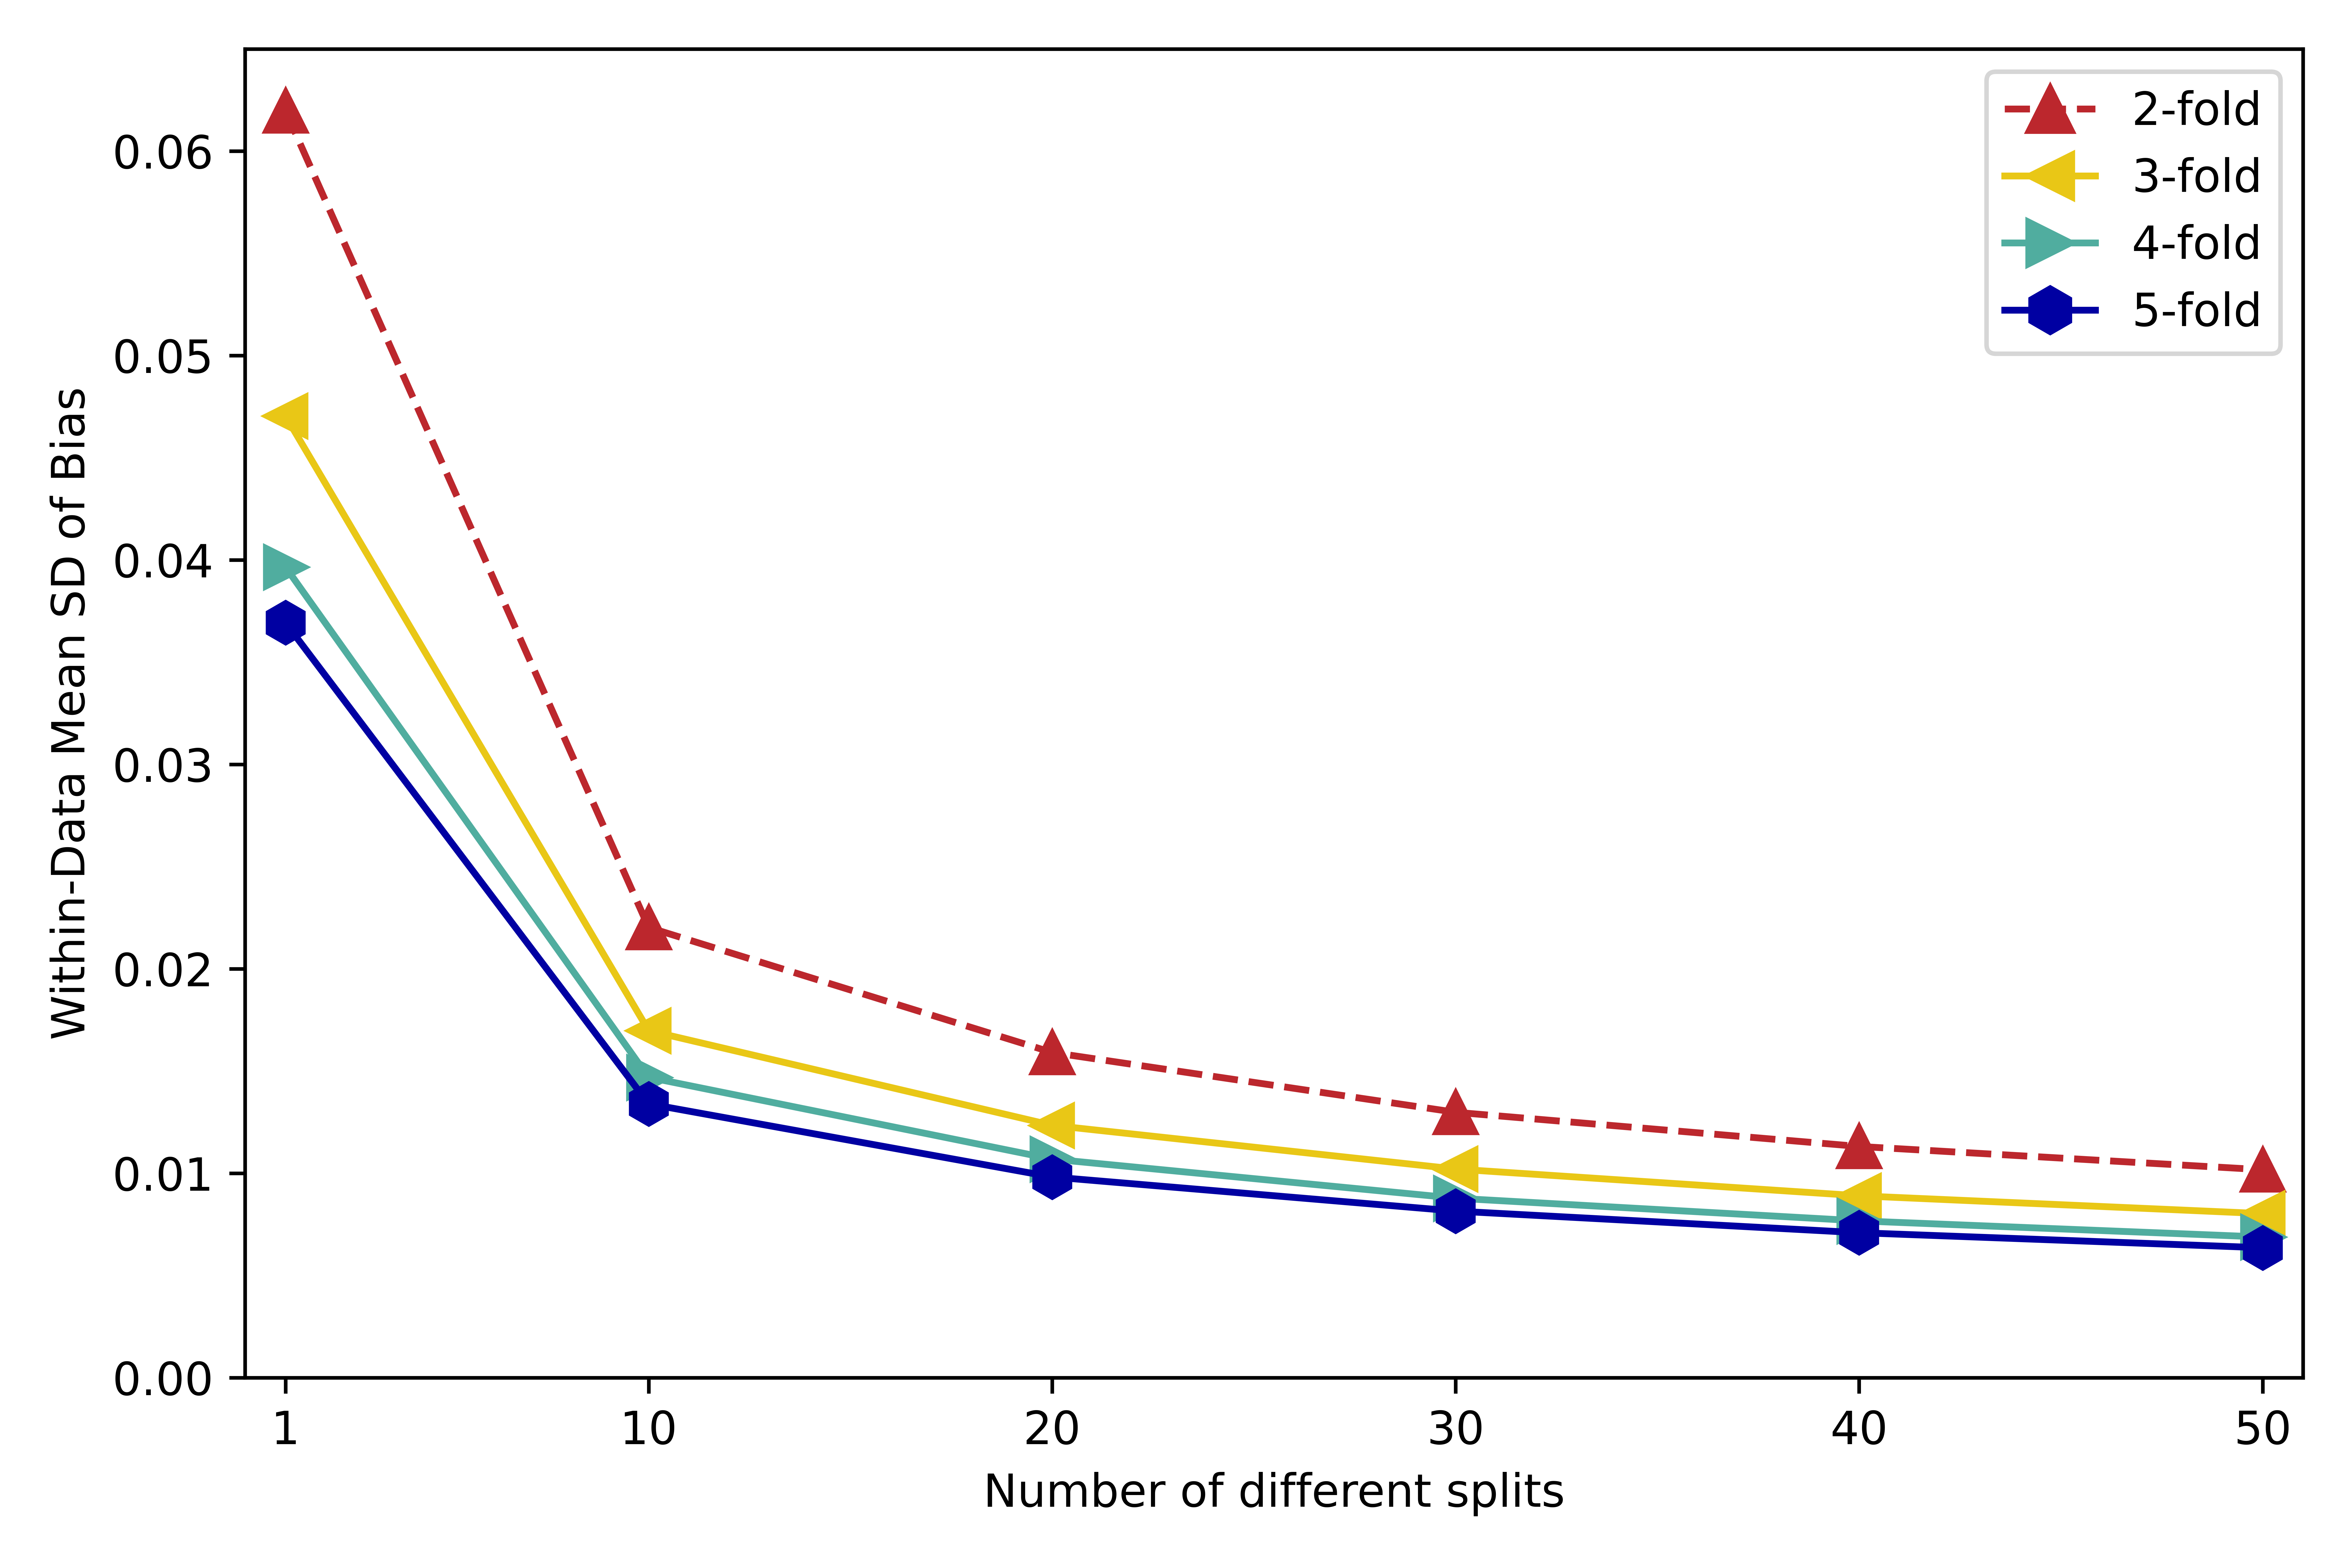
\includegraphics[width=0.99\linewidth]{images/results_sd_bias.png}
	\end{center}
\end{frame}

\begin{frame}{Results -- Standard Error Estimate}
	\begin{center}
		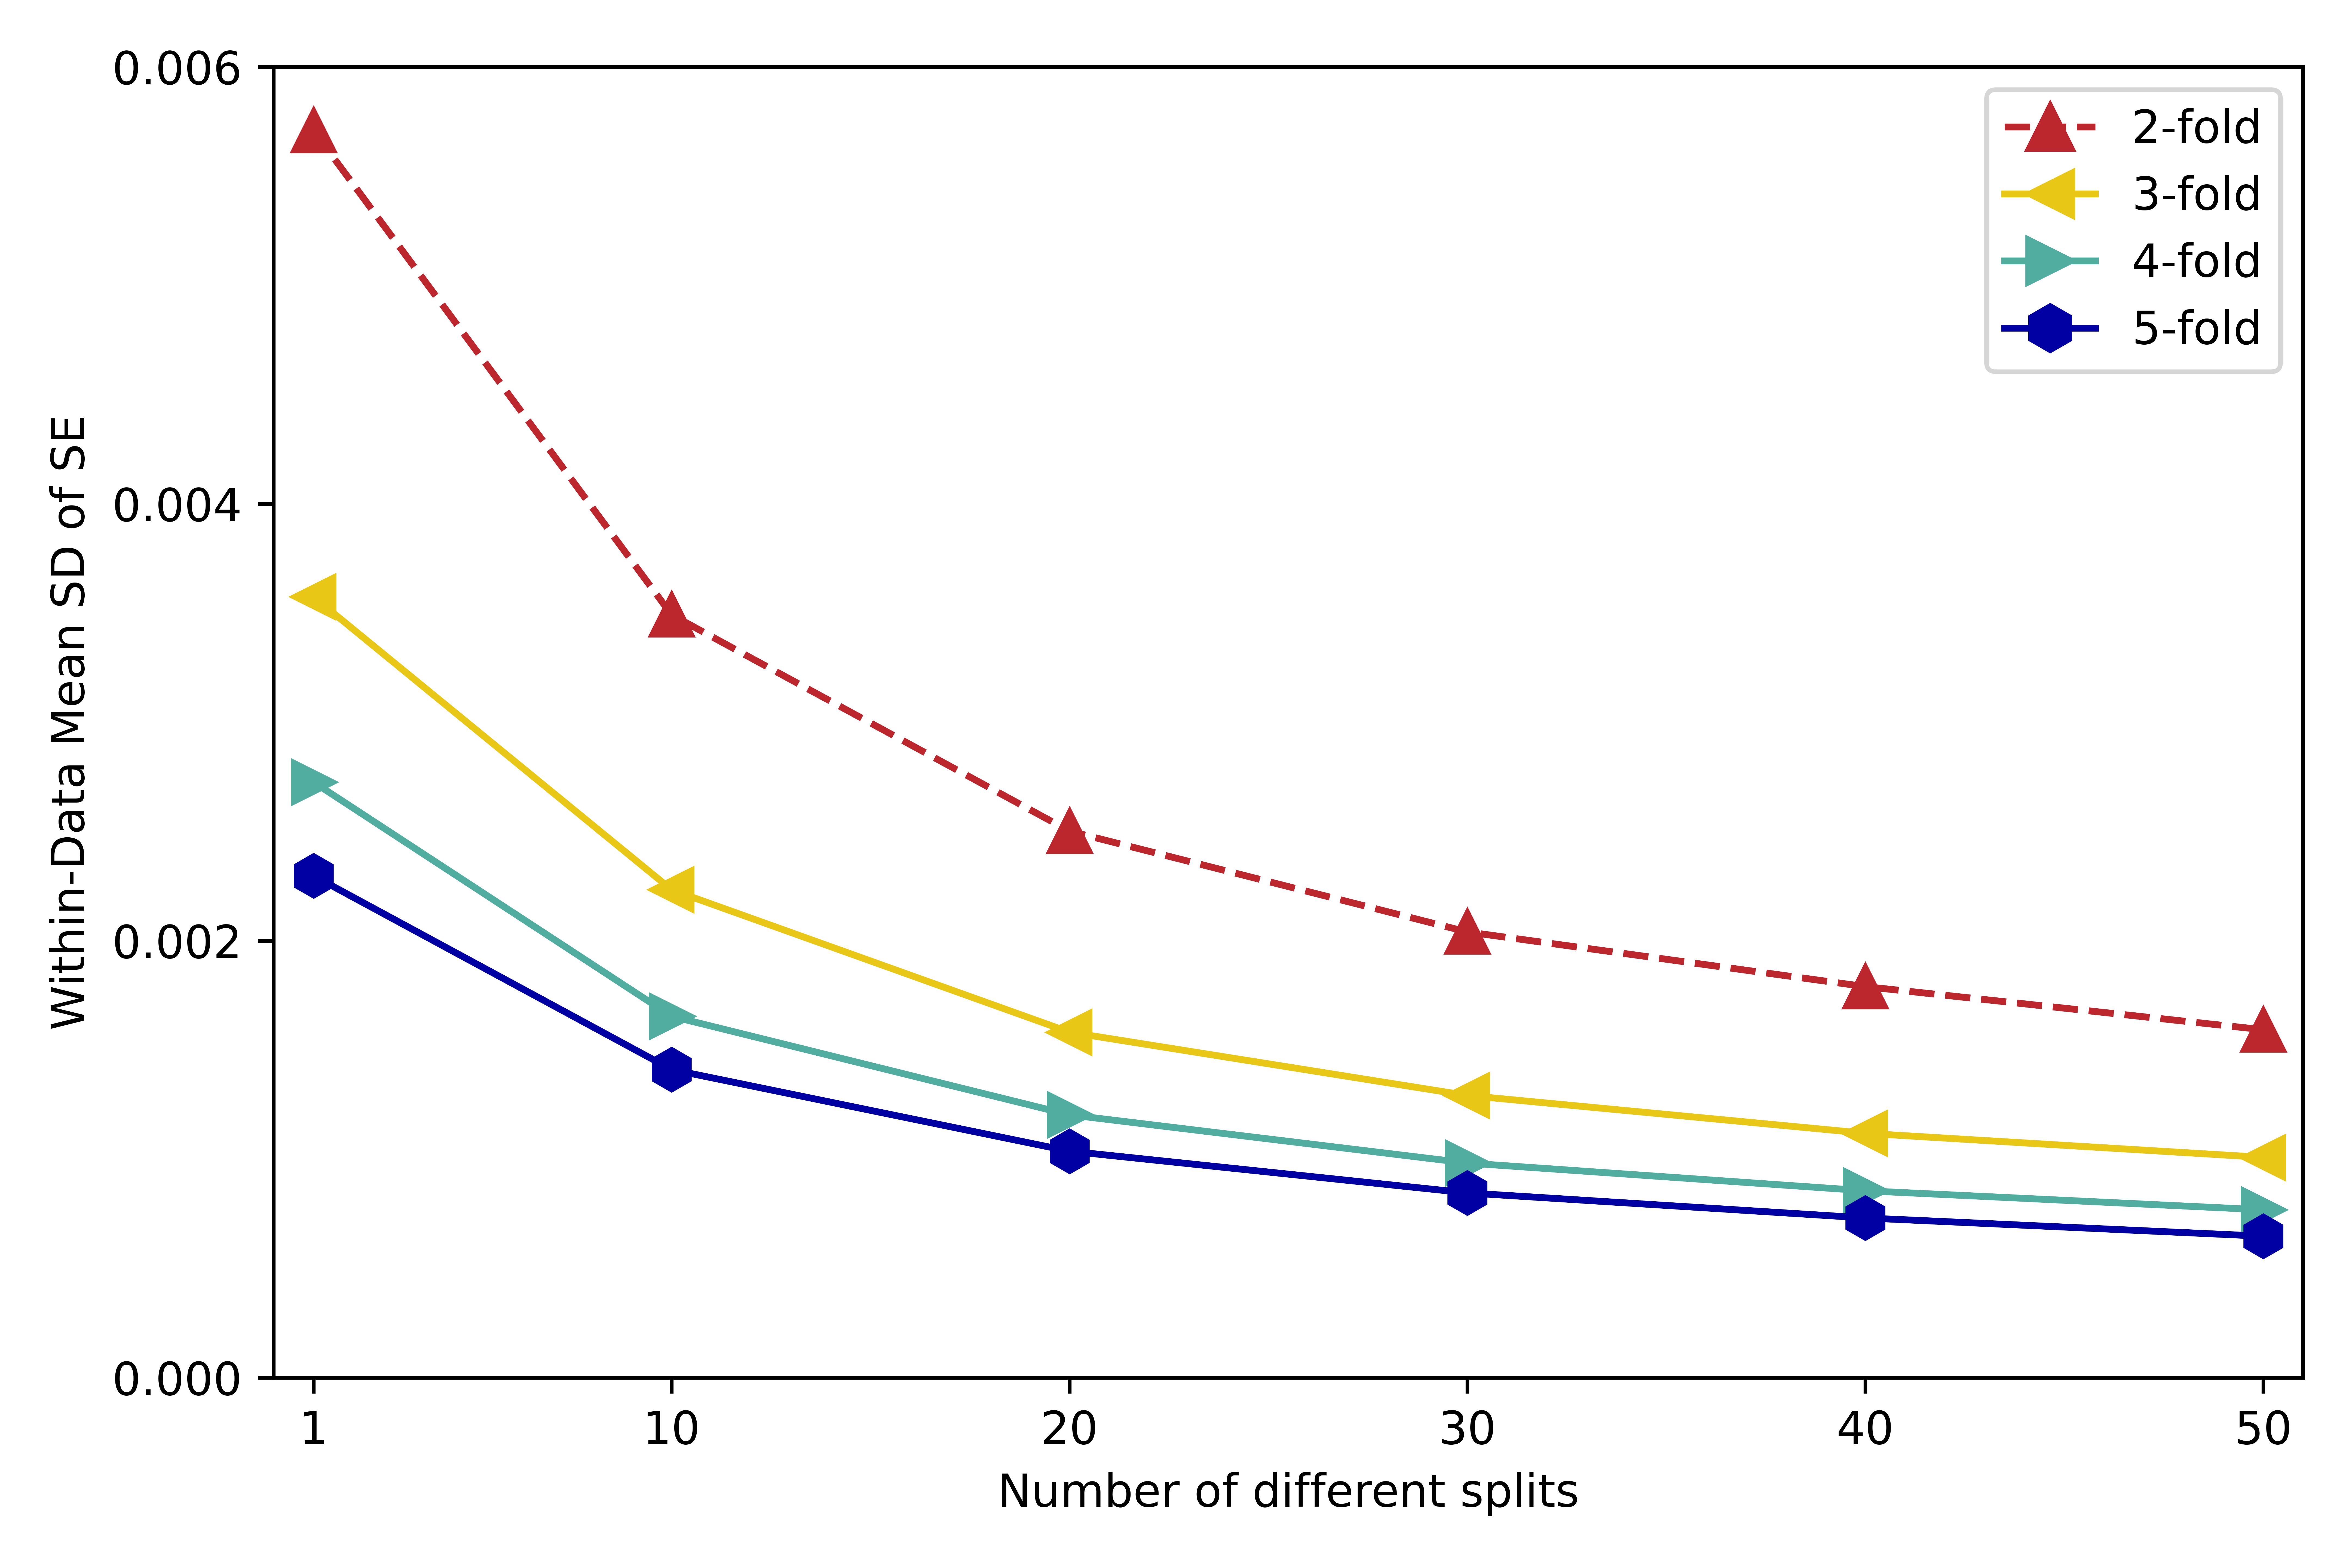
\includegraphics[width=0.99\linewidth]{images/results_sd_se.png}
	\end{center}
\end{frame}

\section{Conclusions}

\begin{frame}{Summary}
	RNG seed dependence is unacceptable
	~\\~\\	
	Steps can be taken to reduce RNG seed dependence
	\begin{itemize}
		\item Number of splits
		\item Increasing number of folds
		\item Easy to implement but computationally intense
	\end{itemize}
\end{frame}

\begin{frame}{Thank you}
	\begin{center}
		{\Huge Questions?}
	\end{center}
	~\\~\\
	\begin{center}
		\small
		\faEnvelope \quad pzivich@unc.edu \qquad \quad 
		\faGithub \quad pzivich \qquad \quad
		\faHashtag \quad pausalz@bsky.social
	\end{center}
	~\\~\\
	Zivich ``Commentary: The Seedy Side of Causal Effect Estimation with Machine Learning" \textit{Epidemiology} 2024; 35(6):787-790
\end{frame}

\end{document}